\documentclass{article}
\usepackage{tikz} 
\usepackage[utf8]{inputenc}
\usepackage{amsmath}
\usepackage{listings}
\usepackage{amsfonts}
\usepackage{amssymb}
\usepackage{amsthm}
\usepackage{tabularx}
\usepackage{enumitem}
\usepackage{algorithm}% http://ctan.org/pkg/algorithm
\usepackage[noend]{algpseudocode}% http://ctan.org/pkg/algorithmicx
\usepackage[margin=0.7in]{geometry}
\usepackage{tikz}
\usepackage{subcaption}
\usepackage{graphicx}
\usepackage{multicol,caption}

\usetikzlibrary{arrows,positioning} 
\thispagestyle{empty}
\pgfarrowsdeclarecombine{ring}{ring}{}{}{o}{o}
\DeclareMathOperator{\ringarrow}{\raisebox{0.5ex}{\tikz[baseline]{\draw[ring->](0,0)--(2em,0);}}}

\tikzset{
    %Define standard arrow tip
    >=stealth',
    %Define style for boxes
    observed/.style={
           rectangle,
           rounded corners,
           draw=black, thick,
           minimum width=2.5em,
           minimum height=2.5em,
           font=\footnotesize,
           text centered,
           },
     latent/.style={
           rectangle,
           rounded corners,
           draw=black, thick, dashed,
           minimum width=2.5em,
           minimum height=2.5em,
           font=\footnotesize,
           text centered,
           fill=black!10!white
           },
            empty/.style={
           circle,
           rounded corners,
           minimum width=.5em,
           minimum height=.5em,
           font=\footnotesize,
           text centered,
           },
    % Define arrow style
    pil/.style={
           o->,
           thick,
           shorten <=2pt,
           shorten >=2pt,},
    sh/.style={ shade, shading=axis, left color=red, right color=green,
    shading angle=45 }
    
}

\renewcommand{\P}[1]{\operatorname{P}\left\{#1\right\}}
\newcommand{\E}[1]{\mathbb E\left[#1\right]}
\newcommand{\set}[1]{\left\{#1\right\}}
\newcommand{\eqn}[1]{\begin{align}#1\end{align}}
\newcommand{\eq}[1]{\begin{align*}#1\end{align*}}

\theoremstyle{plain}
\newtheorem{theorem}{Theorem}
\newtheorem{proposition}[theorem]{Proposition}
\newtheorem{lemma}[theorem]{Lemma}
\newtheorem{corollary}[theorem]{Corollary}
\theoremstyle{definition}
\newtheorem{definition}[theorem]{Definition}
\newtheorem{assumption}[theorem]{Assumption}
\newtheorem{remark}[theorem]{Remark}
\newtheorem{example}[theorem]{Example}
   
\begin{document}

\section{Contextual bandit related problems}

The confounded causal bandit problem, as introduced by \cite{Bareinboim2015}, is illustrated in figure \ref{fig:causalStructure}. At each timestep $t$, $u_t$, $\boldsymbol{r_t}$ and $a'_t$ are generated stochastically. Only $a'$ is observed. The algorithm then selects an action $a_t \in \set{1,...,k}$ and observes the corresponding reward $r_{a_t}$. $a' \in \set{1,...,k}$ corresponds to the action that would have been selected if action choice were not decided by the algorithm. This corresponds exactly to an instance of the standard stochastic contextual bandit problem, with context $x_t = a'_t$. See the following definitions from \cite{Langford2008}

\begin{figure}[h]
\centering
\caption{Causal model for confounded bandits}
\label{fig:causalStructure}
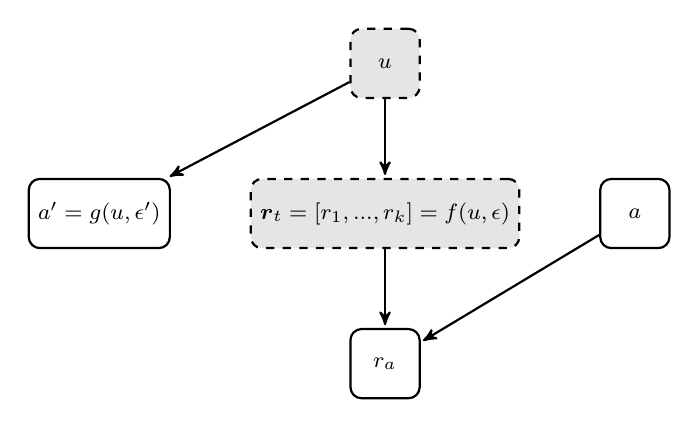
\begin{tikzpicture}[->,>=stealth',shorten >=1pt,auto,node distance=1cm,
  thick,main node/.style={observed}, hidden/.style={empty}]
 %nodes
\node[latent](1){$u$};
\node[latent, below =of 1](2){$\boldsymbol{r}_t = [r_1,...,r_k] = f(u,\epsilon)$};
\node[main node,  right=of 2](3){$a$};
\node[main node,  left=of 2](4){$a' = g(u,\epsilon')$};
\node[main node,  below=of 2](5){$r_a$};
 \path[every node/.style={font=\sffamily\small}]
    (1) edge (2) edge (4)
    (2) edge (5)
    	(3) edge (5);
\end{tikzpicture}
\end{figure}



\begin{definition}[Contextual bandit problem]
In a contextual bandits problem, there is a distribution
$P$ over $(x, r_1, ..., r_k)$, where $x$ is context, $a \in \set{1...k}$ is one of the $k$ arms to be pulled,and $r_a \in [0,1]$ is the reward for arm $a$. The problem is a repeated game: on each round, a sample
$(x, r_1, ..., r_k)$ is drawn from $P$, the context $x$ is announced, and then for precisely one arm a chosen
by the player, its reward $r_a$ is revealed.
\end{definition}

\begin{definition}[Contextual bandit algorithm] A contextual bandit algorithm $\mathcal{B}$ determines an arm $a \in \set{1...k}$ to pull at each timestep $t$, based on the previous observation sequence $(x_1, a_1,r_{a,1})$, and the current context $x_t$.
\end{definition}

\begin{definition}[Regret] Assume we have a hypothosis set $\mathcal{H}$ consisting of hypotheses $h: \mathcal{X} \rightarrow \set{1,...,k}$
The regret of an algorithm $\mathcal{B}$ with respect to $h$ is
\eq{
\Delta R(h,\mathcal{B},T) = T \E{r_{h(x)}} - \E{\sum_{t=1}^T r_{\mathcal{B}(x),t}}
}
and the (psudo) regret of $\mathcal{B}$ with respect to the hypothesis space $\mathcal{H}$ is 
\eq{
\Delta R(\mathcal{H},\mathcal{B},T) = \sup_{h \in \mathcal{H}}\Delta R(h,\mathcal{B},T)
}
\end{definition}

Note - that the definition of a contextual bandit problem does not require that the context is a direct cause of the outcome.


\section{Questions}
Two questions arose in our discussion of this problem.
\subsection{Are noisy features more problematic in the bandit setting}
Intuitively adding features that are noisy (ie only weakly related to the target) is more problematic in the bandit setting than in the batch learning setting because in batch learning, we can apply feature selection or regularization and tune it via cross-validation. It is unclear how to do this (or model/parameter selection in general) in the contextual bandit setting.

Some more concrete version of the question. 
\begin{itemize}
\item Assume we are in the confounded causal bandit setting and $Y_t \in \set{0,1}$ Suppose we make no assumptions about $f$ track the rewards separately for each value of $a'_t$. Under what conditions (on $g$, $f$ and $T$) does including the context have lower regret than applying a standard bandit algorithm. 

\item What happens if we add context that is entirely uncorrelated with the target. Ie a contextual bandit where the context $\boldsymbol{x} = [x_1,...x_m]$ but $Y = f(x_1...x_d,\epsilon)$ where $d < m$. How does the regret depend on $m$ and $d$ (with or witout assumptions such as linearity on f). This paper may be relevant \cite{abbasi2012online}.

\item How can we quantify dependence without reference to a model? KL divergence between $P(X,Y)$ and $P(Y)$ averaged over $X$? max over possible kernelized fits (as in kernelized conditional independence testing)? For linear models, all captured in the inverse correlation matrix.  

\end{itemize}


\subsection{How should we represent the context} 
In the confounded bandit problem, $x$ is discrete with $k$ unique values. We could:
\begin{enumerate}
\item Treat it as a categorical feature
\item Treat each value of $x$ as a task and apply a multi-task algorithm
\item Treat it as a structured output prediction problem (how)?
\end{enumerate}

Its hard to find a quantitative definition of multi-task learning. One variant involves parameterising models for each task in terms of some weights and putting a joint constraint over the weights of all tasks \ref{}. This is equivalent to treating the tasks as a categorical variable and regularizing for some choices of constraint, and regularizer (given conditions on the loss-function). 

The feature-mappings for structured output prediction involve the label - so at first pass this seems different -but I haven't properly understood how this approach works and how the problem can be represented as a structured output prediction problem.

\bibliography{Reinforcment-contextual}
\bibliographystyle{apalike}
\end{document}